% ******************************* Thesis Appendix D ********************************
\chapter{} 
\label{app:MATLABRoll}

\graphicspath{{Appendix4/Figs/}}

\renewcommand{\thefigure}{D\arabic{figure}}

\setcounter{figure}{0}

The following 4 figures are the results of the roll lag testing performed as part of the path planning task testing. The four configurations are:

\begin{enumerate}
	\item 65\degree\  maximum roll angle, airspeed of 20 metres per second
	\item 65\degree\  maximum roll angle, airspeed of 10 metres per second
	\item 32.5\degree\  maximum roll angle, airspeed of 20 metres per second
	\item 32.5\degree\  maximum roll angle, airspeed of 10 metres per second
\end{enumerate}

The figures appear in the order the configurations are listed here.

\begin{sidewaysfigure}[htbp!] 
\centering    
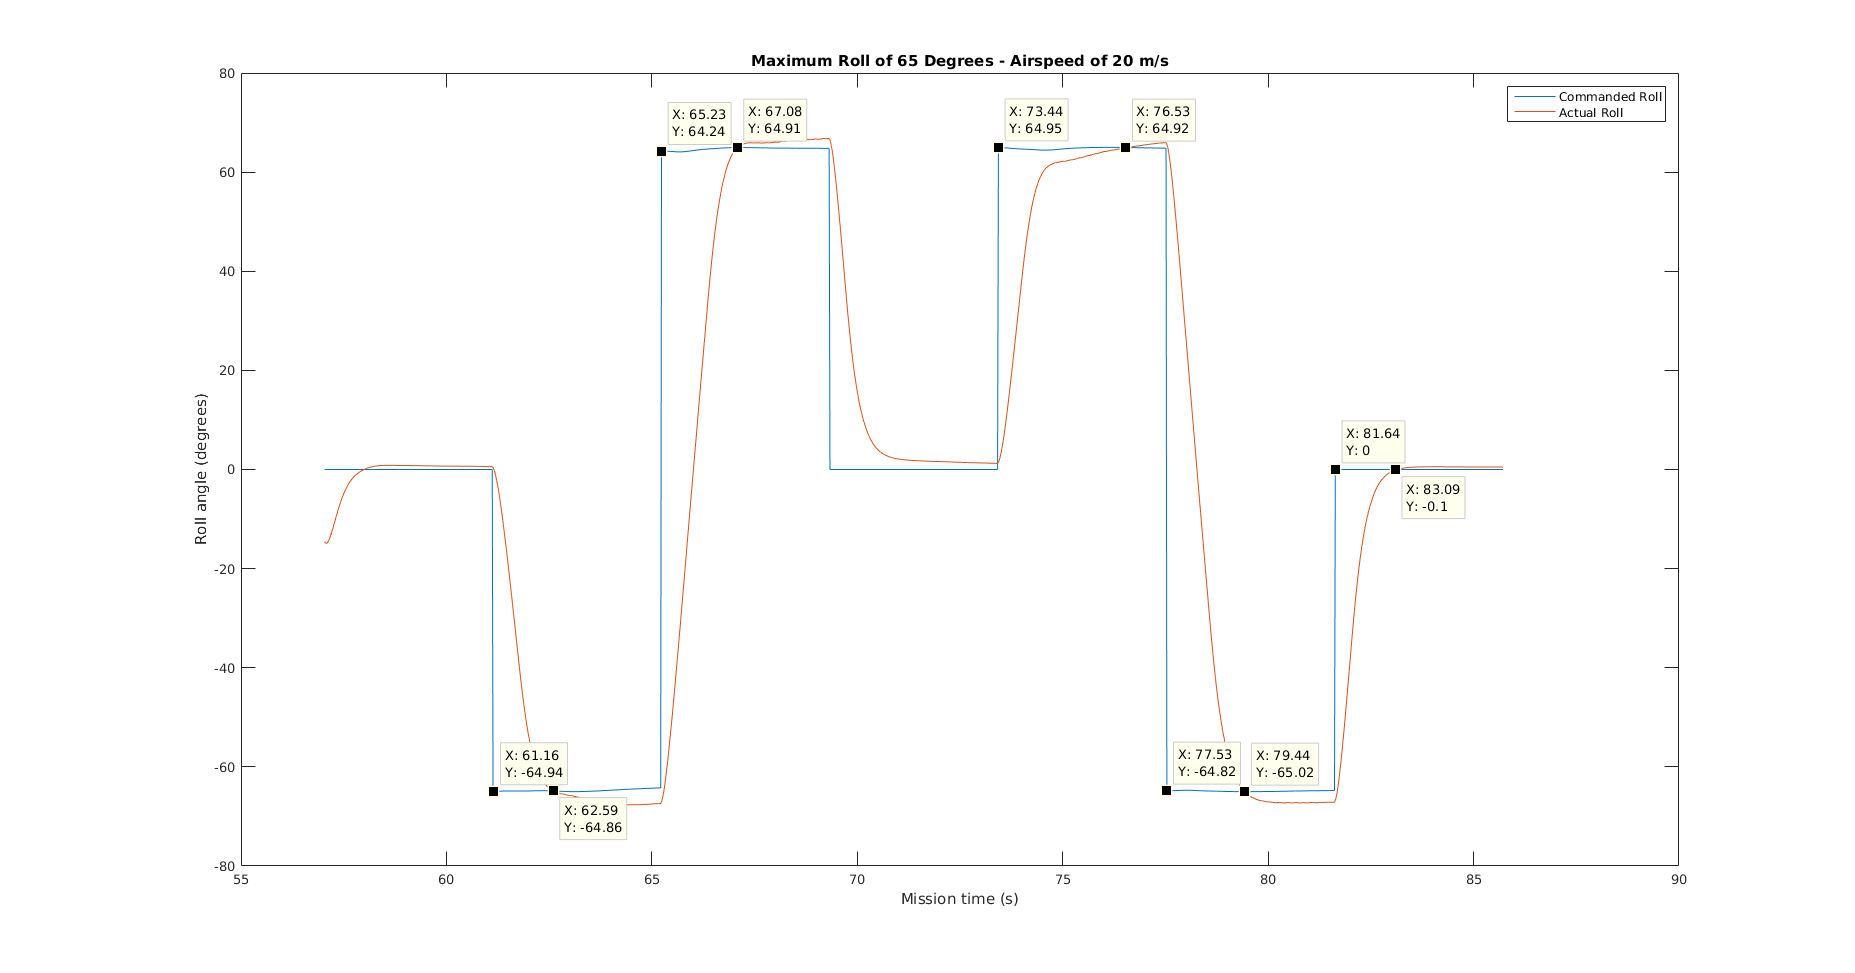
\includegraphics[scale=0.5]{65_20_cursors}
\caption{A comparison of the commanded roll angle with the actual roll angle over time. Flying with a 65\degree\  maximum roll angle, and at an airsped of 20 metres per second}
\end{sidewaysfigure}

\begin{sidewaysfigure}[htbp!] 
\centering    
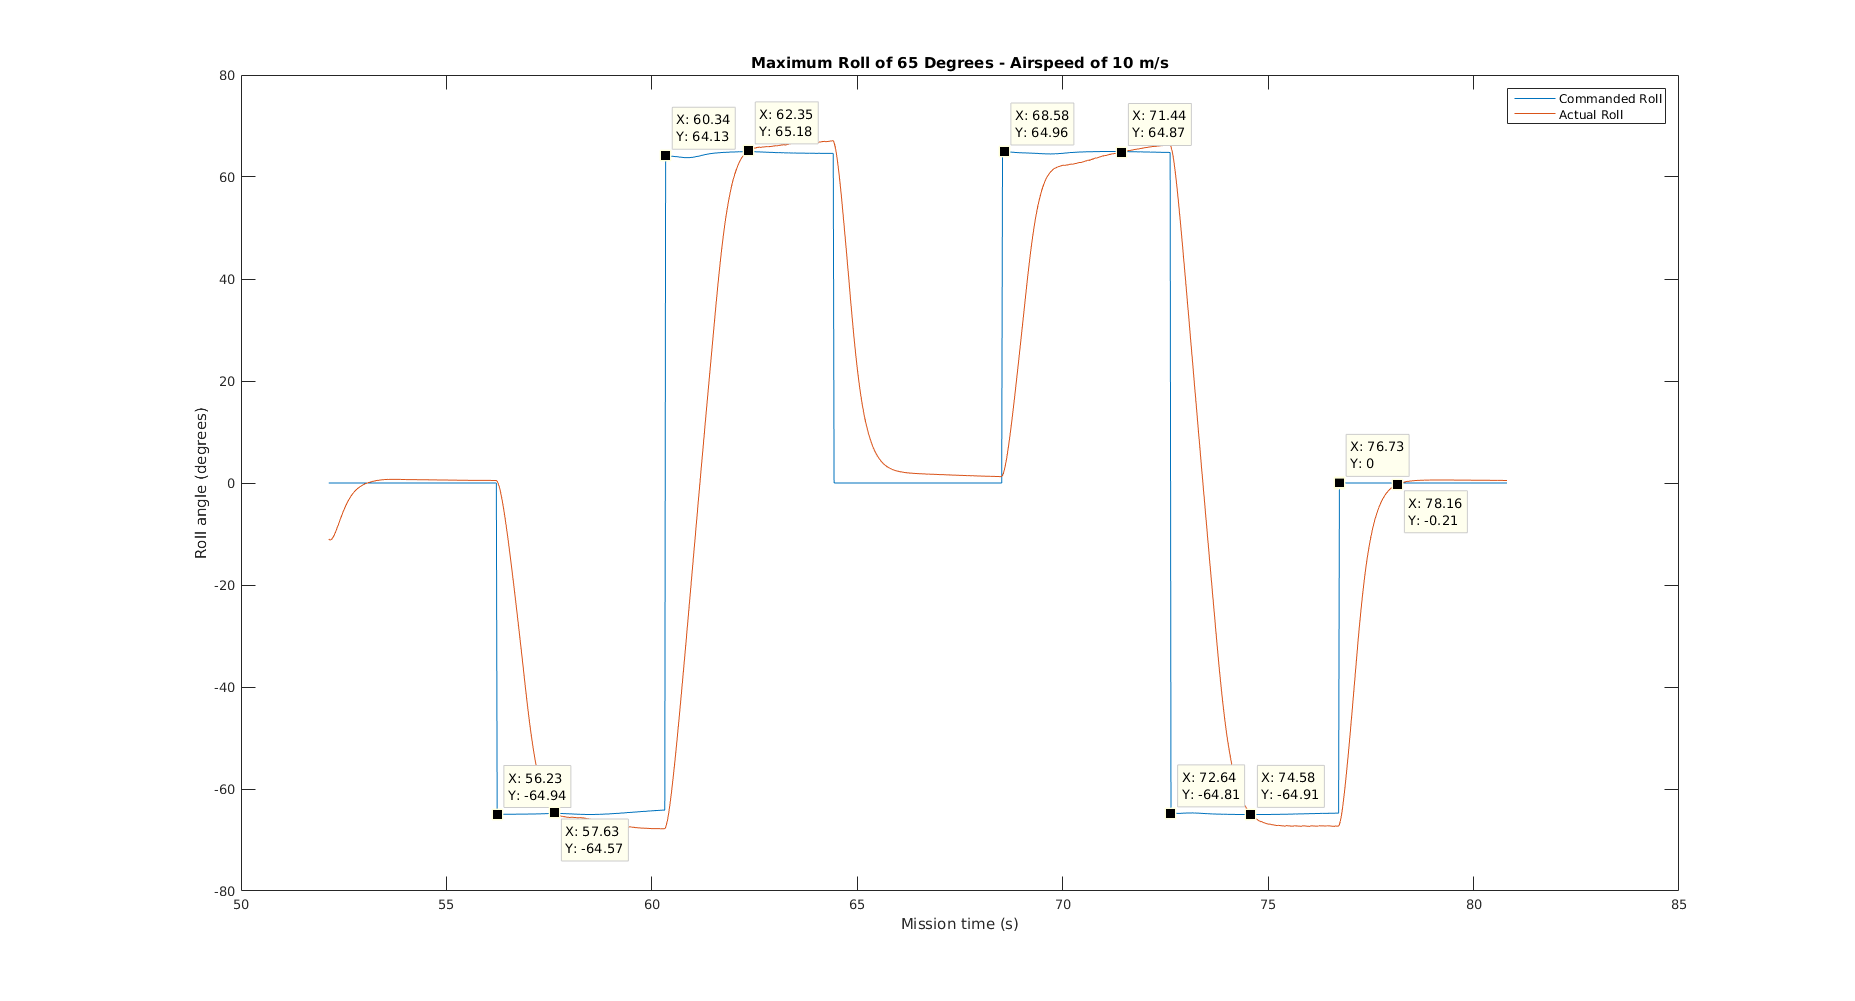
\includegraphics[scale=0.5]{65_10_cursors}
\caption{A comparison of the commanded roll angle with the actual roll angle over time. Flying with a 65\degree\  maximum roll angle, and at an airsped of 10 metres per second}
\end{sidewaysfigure}

\begin{sidewaysfigure}[htbp!] 
\centering    
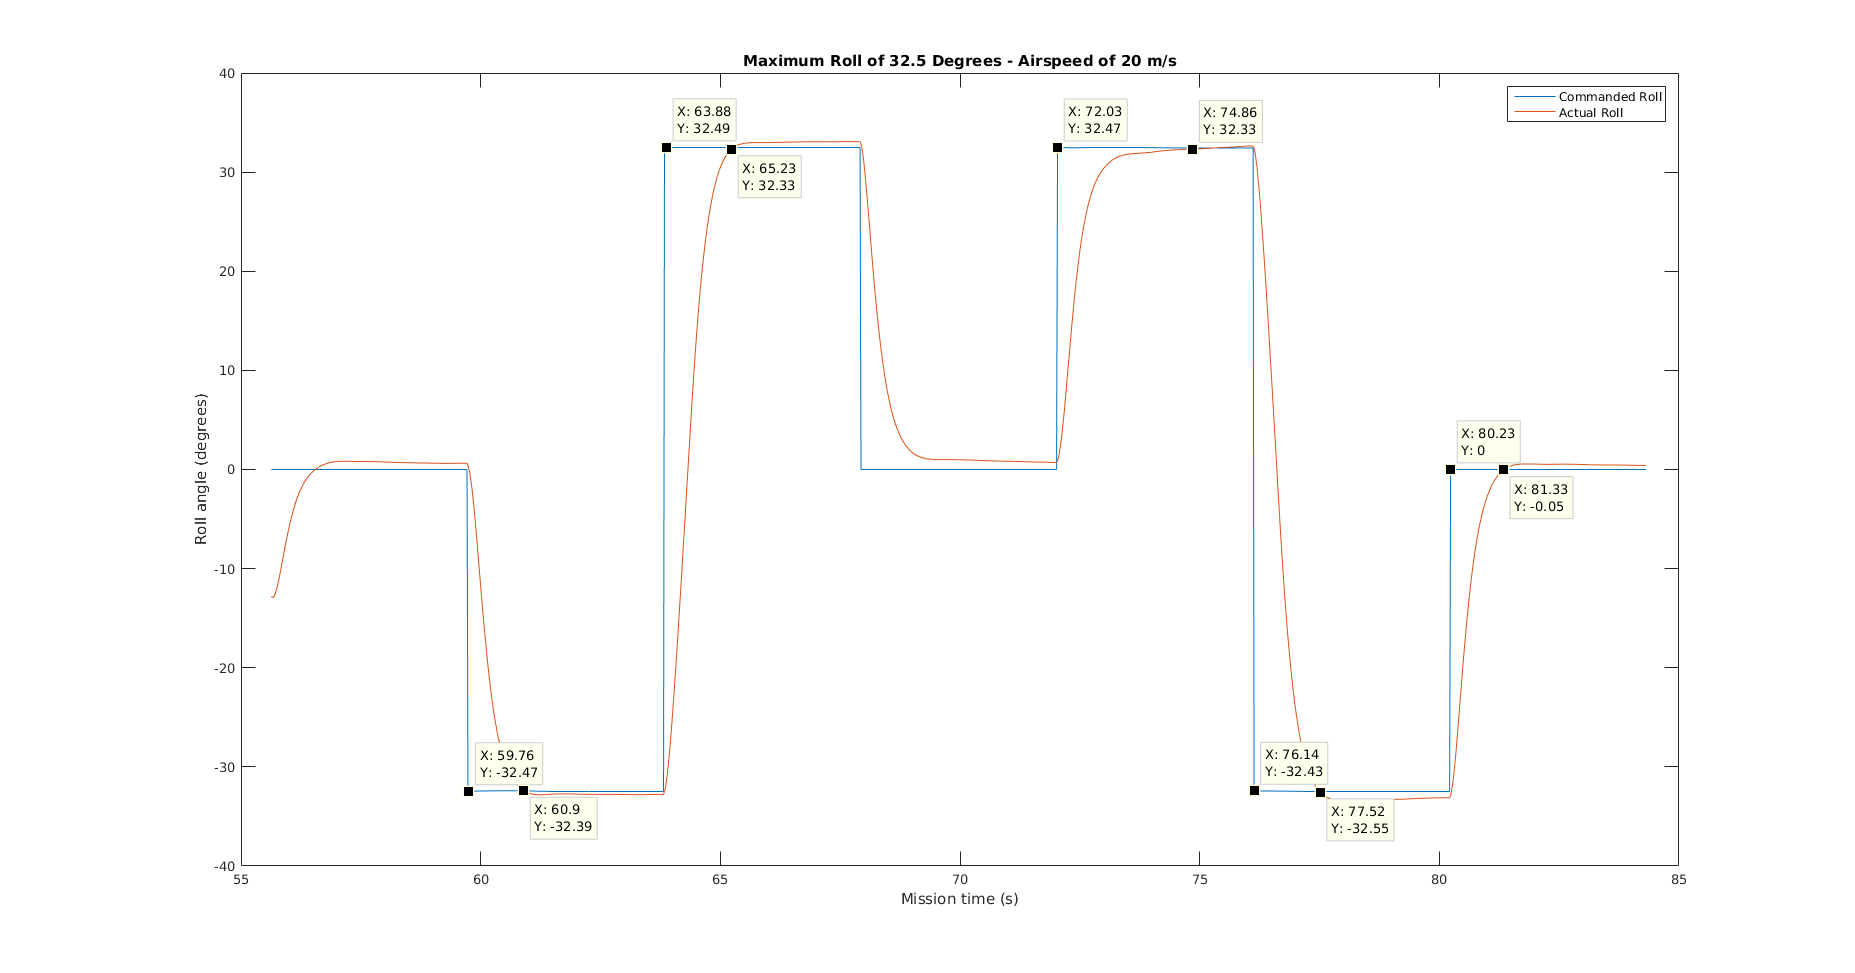
\includegraphics[scale=0.5]{32_20_cursors}
\caption{A comparison of the commanded roll angle with the actual roll angle over time. Flying with a 32.5\degree\  maximum roll angle, and at an airsped of 20 metres per second}
\end{sidewaysfigure}

\begin{sidewaysfigure}[htbp!] 
\centering    
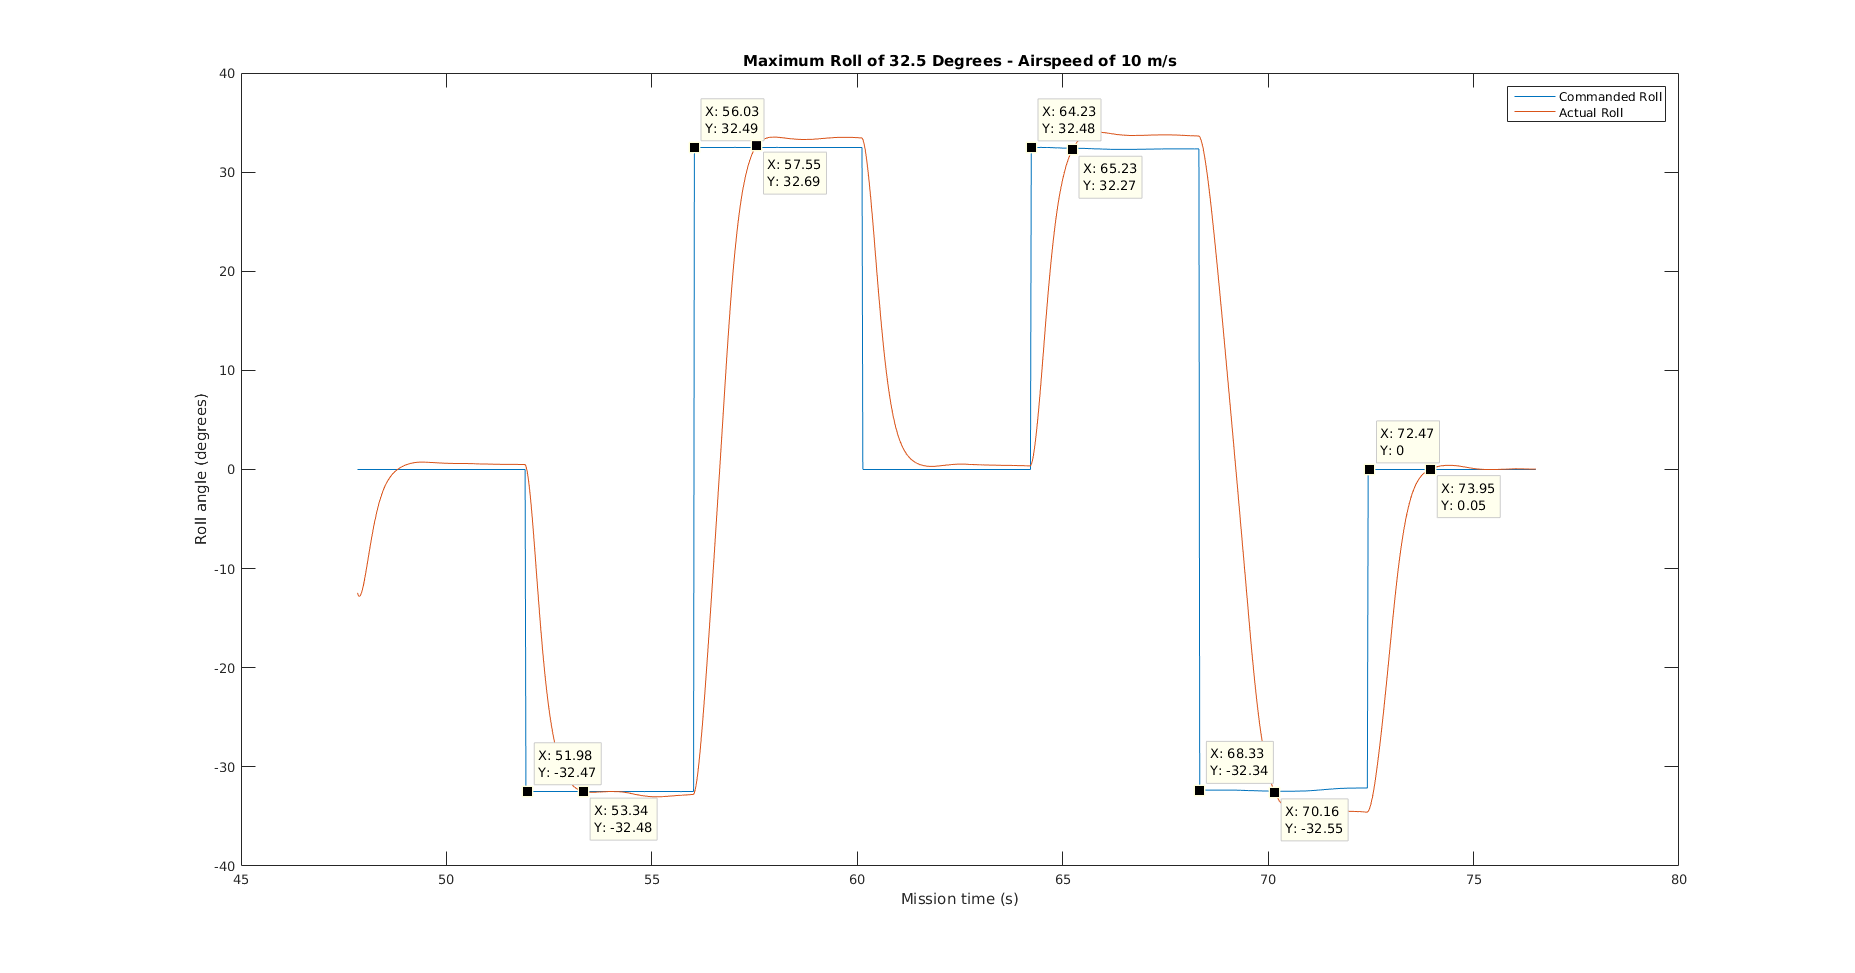
\includegraphics[scale=0.5]{32_10_cursors}
\caption{A comparison of the commanded roll angle with the actual roll angle over time. Flying with a 32.5\degree\  maximum roll angle, and at an airsped of 10 metres per second}
\end{sidewaysfigure}